%%%%%%%%%%%%%%%%%%%%%%%%%%%%%%%%%%%%%%%%%
% Large Colored Title Article
% LaTeX Template
% Version 1.1 (25/11/12)
%
% This template has been downloaded from:
% http://www.LaTeXTemplates.com
%
% Original author:
% Frits Wenneker (http://www.howtotex.com)
%
% License:
% CC BY-NC-SA 3.0 (http://creativecommons.org/licenses/by-nc-sa/3.0/)
%
%%%%%%%%%%%%%%%%%%%%%%%%%%%%%%%%%%%%%%%%%

%----------------------------------------------------------------------------------------
%	PACKAGES AND OTHER DOCUMENT CONFIGURATIONS
%----------------------------------------------------------------------------------------

\documentclass[DIV=calc, paper=letterpaper, fontsize=11pt, twocolumn]{scrartcl}	 % A4 paper and 11pt font size

\usepackage{lipsum} % Used for inserting dummy 'Lorem ipsum' text into the template
\usepackage[english]{babel} % English language/hyphenation
\usepackage[protrusion=true,expansion=true]{microtype} % Better typography
\usepackage{amsmath,amsfonts,amsthm} % Math packages
\usepackage[svgnames]{xcolor} % Enabling colors by their 'svgnames'
\usepackage[hang, small,labelfont=bf,up,textfont=it,up]{caption} % Custom captions under/above floats in tables or figures
\usepackage{booktabs} % Horizontal rules in tables
\usepackage{fix-cm}	 % Custom font sizes - used for the initial letter in the document
\usepackage{subfig}
\usepackage{graphicx}
\graphicspath{{Figures/}} % Set the default folder for images

\usepackage{sectsty} % Enables custom section titles
\allsectionsfont{\usefont{OT1}{phv}{b}{n}} % Change the font of all section commands

\usepackage{fancyhdr} % Needed to define custom headers/footers
\pagestyle{fancy} % Enables the custom headers/footers
\usepackage{lastpage} % Used to determine the number of pages in the document (for "Page X of Total")

% Headers - all currently empty
\lhead{}
\chead{}
\rhead{}

% Footers
\lfoot{}
\cfoot{}
\rfoot{\footnotesize Page \thepage\ of \pageref{LastPage}} % "Page 1 of 2"

\renewcommand{\headrulewidth}{0.0pt} % No header rule
\renewcommand{\footrulewidth}{0.4pt} % Thin footer rule

\usepackage{lettrine} % Package to accentuate the first letter of the text
\newcommand{\initial}[1]{ % Defines the command and style for the first letter
\lettrine[lines=3,lhang=0.3,nindent=0em]{
\color{DarkGoldenrod}
{\textsf{#1}}}{}}

%----------------------------------------------------------------------------------------
%	TITLE SECTION
%----------------------------------------------------------------------------------------

\usepackage{titling} % Allows custom title configuration

\newcommand{\HorRule}{\color{DarkGoldenrod} \rule{\linewidth}{1pt}} % Defines the gold horizontal rule around the title

\pretitle{\vspace{-30pt} \begin{flushleft} \HorRule \fontsize{24}{24} \usefont{OT1}{phv}{b}{n} \color{DarkRed} \selectfont} % Horizontal rule before the title

\title{Potentiostat Hardware for USB-Style Sensors} % Your article title

\posttitle{\par\end{flushleft}\vskip 0.5em} % Whitespace under the title

\preauthor{\begin{flushleft}\large \lineskip 0.5em \usefont{OT1}{phv}{b}{sl} \color{DarkRed}} % Author font configuration

\author{Ben Lorenzetti, } % Your name

\postauthor{\footnotesize \usefont{OT1}{phv}{m}{sl} \color{Black} % Configuration for the institution name
BioMicroSystems Laboratory % Your institution

\par\end{flushleft}\HorRule} % Horizontal rule after the title

\date{} % Add a date here if you would like one to appear underneath the title block

%----------------------------------------------------------------------------------------

\begin{document}

\maketitle % Print the title

\thispagestyle{fancy} % Enabling the custom headers/footers for the first page 

%----------------------------------------------------------------------------------------
%	ABSTRACT
%----------------------------------------------------------------------------------------

% The first character should be within \initial{}

\begin{figure}[ht]
\centering
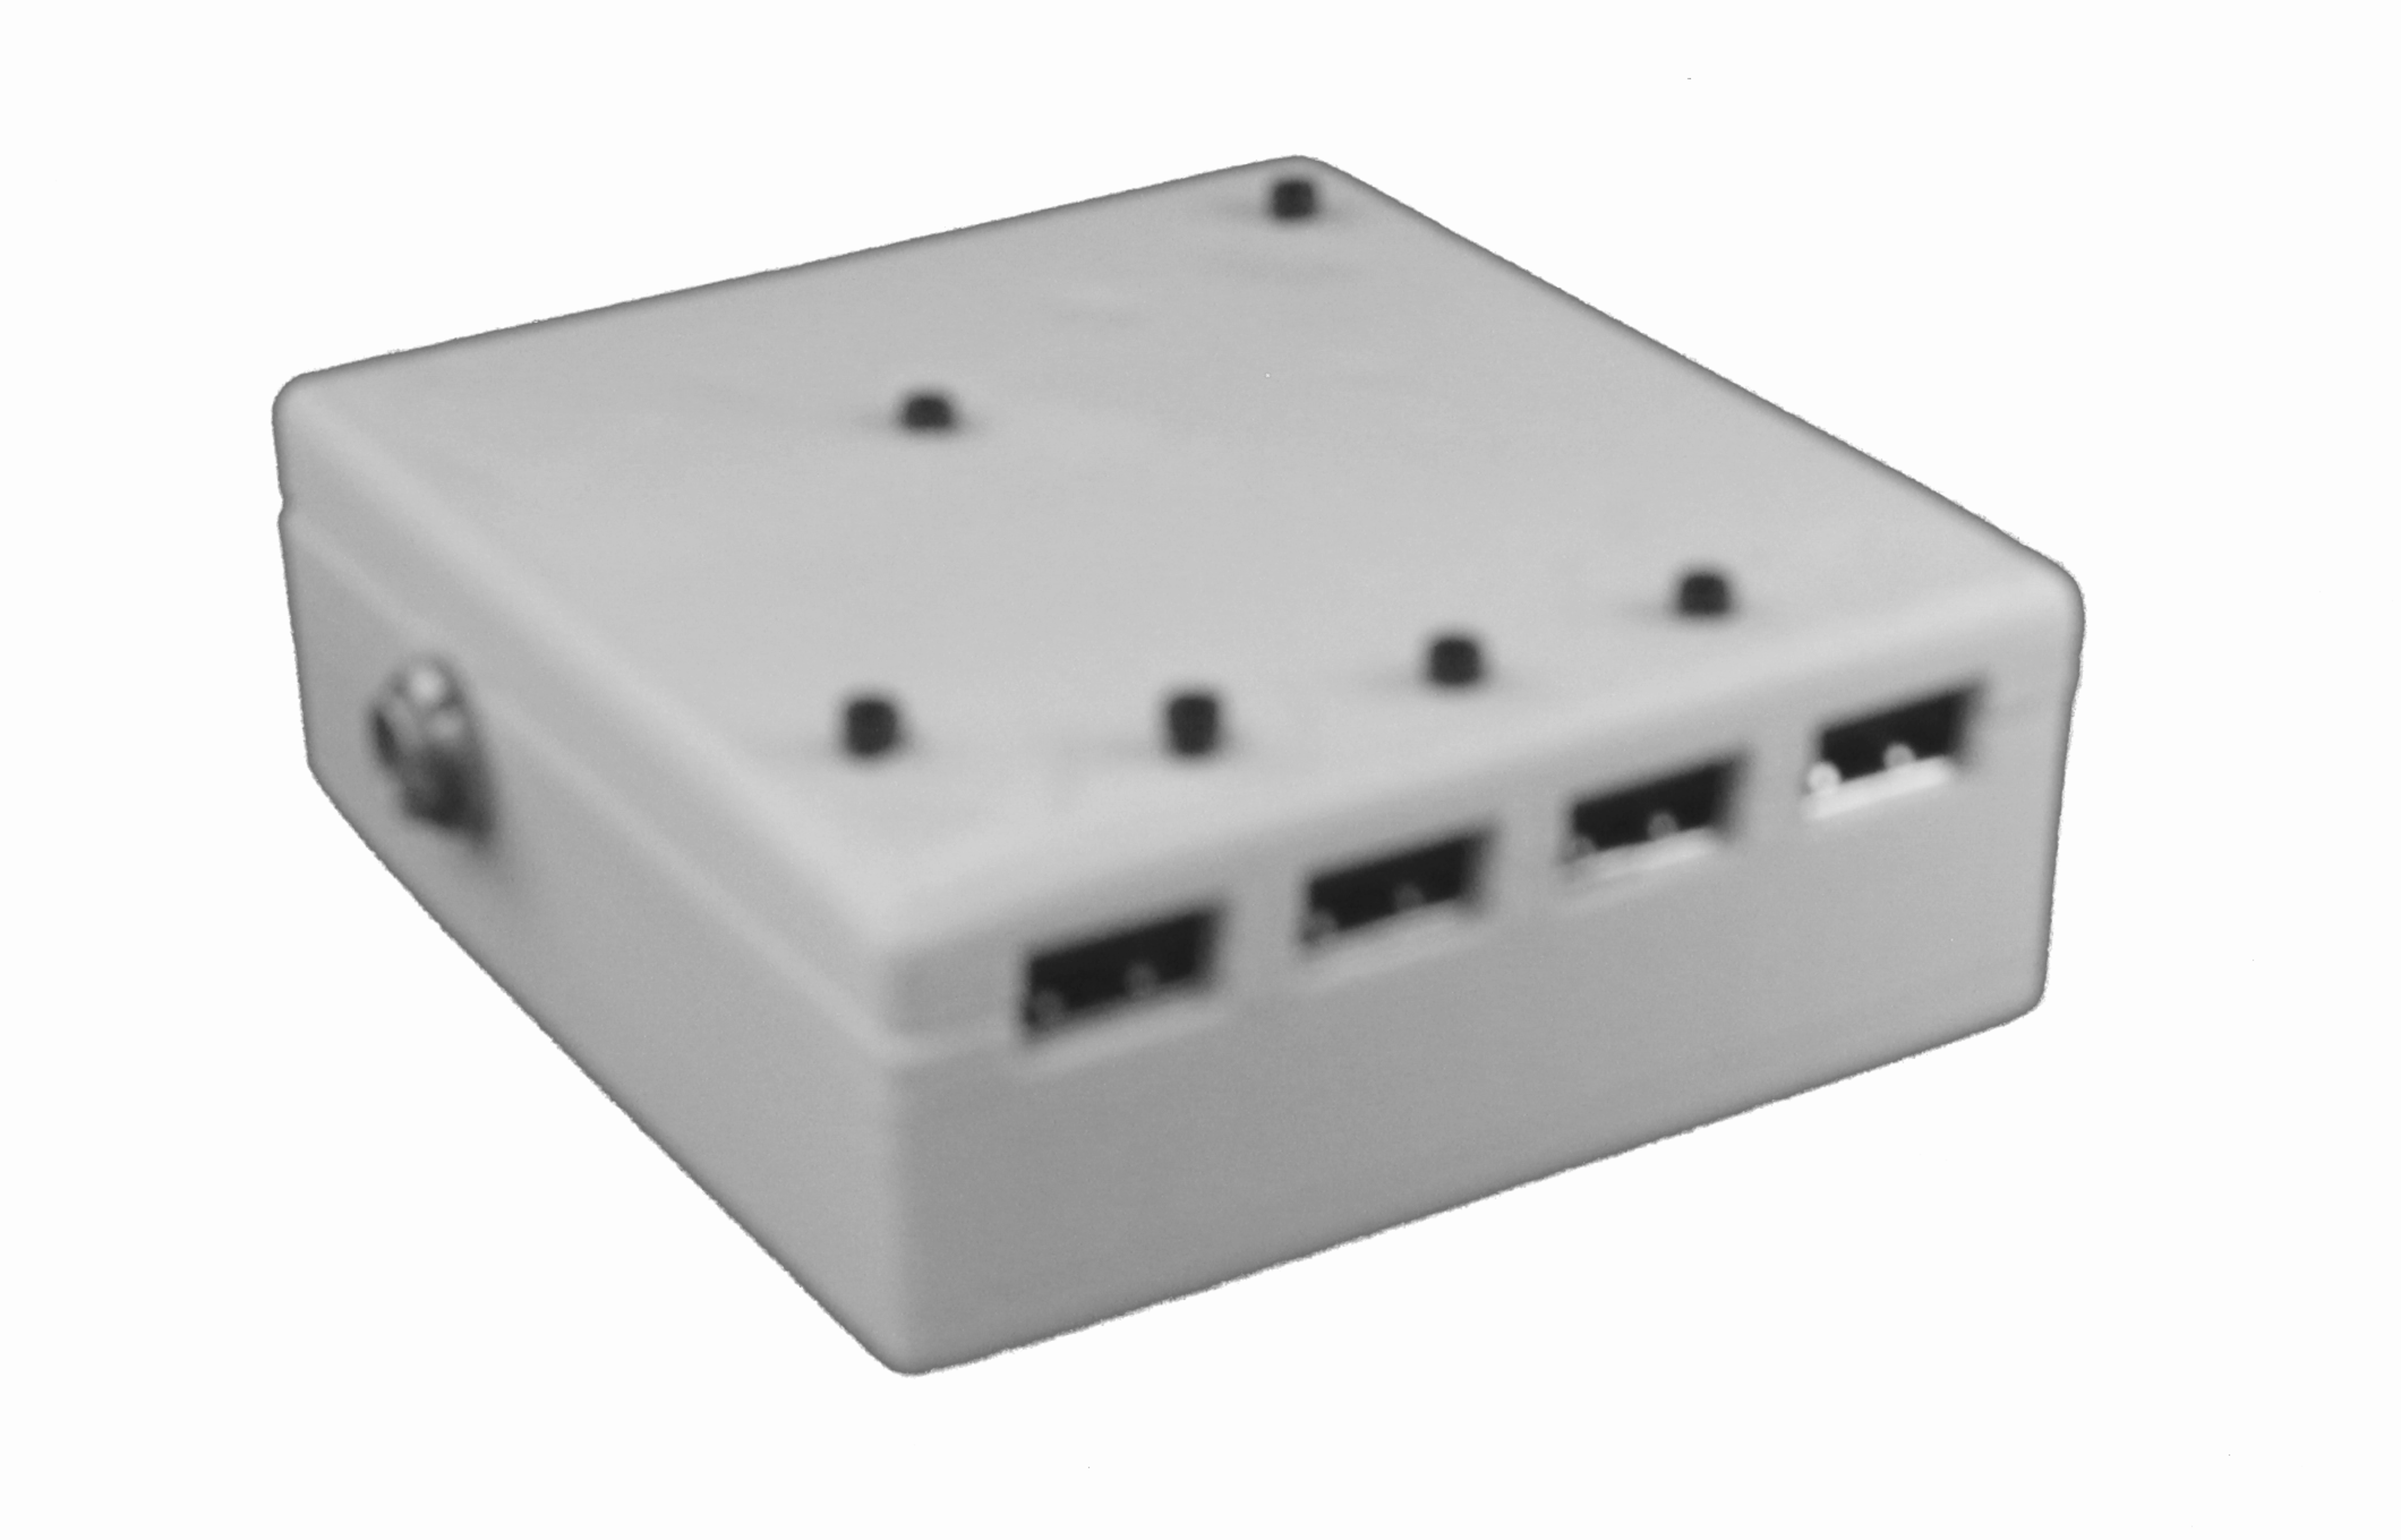
\includegraphics[width=0.6\columnwidth]{complete-assembly}
\end{figure}

\initial{A}\textbf{ portable measurement system was assembled using a commercial potentiostat, a custom circuit board, and a 3D-printed enclosure. The system will help demonstrate the portability and simplicity the electrochemical sensors being developed in BioMicroSystems Lab.}

%----------------------------------------------------------------------------------------
%	ARTICLE CONTENTS
%----------------------------------------------------------------------------------------

\section*{Introduction}

BioMicroSystems (BMS) Lab is developing point-of-care electrochemical sensors for measuring heavy metal concentrations in environmental samples,
such as manganese in lake water \cite{bms-article}.

\begin{figure}[ht]
\centering
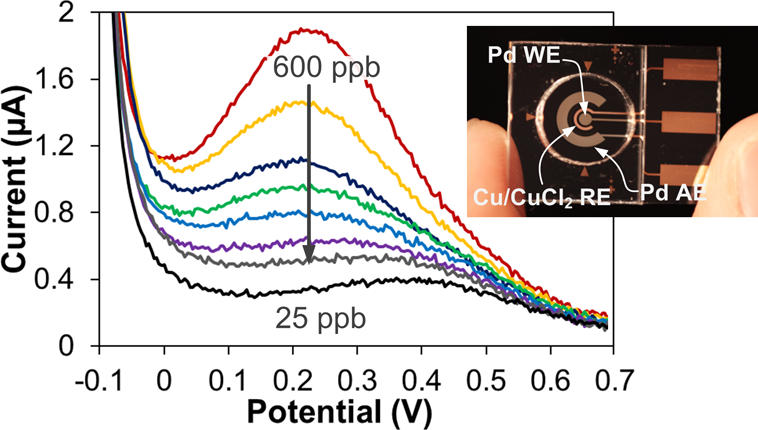
\includegraphics[width=0.9\columnwidth]{analytical-chemistry-copper-electrode}
\caption{Measuring Manganese \cite{bms-article}}
\end{figure}

Three electrodes are inundated in a sample and a potential is applied between two of the electrodes, while
a different pair of two electrodes is used to measure current.
At some applied voltage, an oxidation-reduction reaction occurs between the metal of interest and the working electrode surface.
Charge is emitted as the metal changing oxidation state;
so measuring and integrating the current gives the quantity of metal reagent in the sample.

In a three electrode system, one electrode must be common to both the voltage pair and the current pair,
and this is termed the counter electrode.
For the other two electrodes (reference and working) to accurately separate voltage and current,
they must be virtually grounded by amplifier electronics.
A device which drives the virtual ground, sets a potential, and measures resulting current is called a potentiostat.

\begin{figure}[ht]
\centering
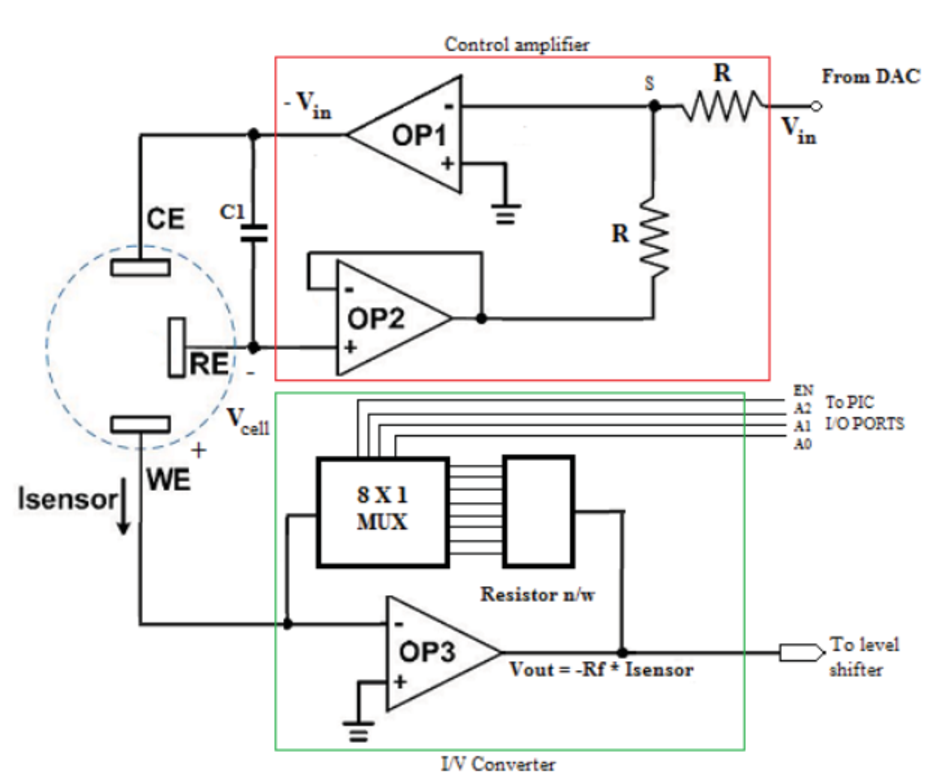
\includegraphics[width=0.9\columnwidth]{zinc-paper-potentiostat}
\caption{Op-Amp Potentiostat \cite{zinc-masters-defense}}
\end{figure}

The possible advantages of the point-of-care electrodes being developed by BMS Lab include
low cost, portability, measurement speed, and simplicity for non-technical operators.
To realize these advantages, a small, portable potentiostat is needed with a simple user interface.

\newpage
%------------------------------------------------

\section*{Method}

An OEM potentiostat board measuring only 2" x 1.35" was purchased from PalmSens, called EmStat.
Also from PalmSens, a Multiplexer was purchased that allows EmStat to switch between multiple sensors.
The EmStat--Multiplexer connection and the external interface towards the sensors are shown in figure \ref{emstat}.

\begin{figure}[tb]
\centering
\subfloat[EmStat Potentiostat]{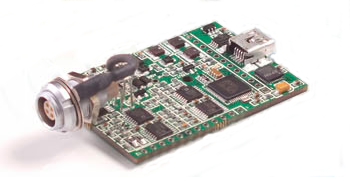
\includegraphics[width=0.45\columnwidth]{EmStat}}	\quad
\subfloat[Pinout Diagram]{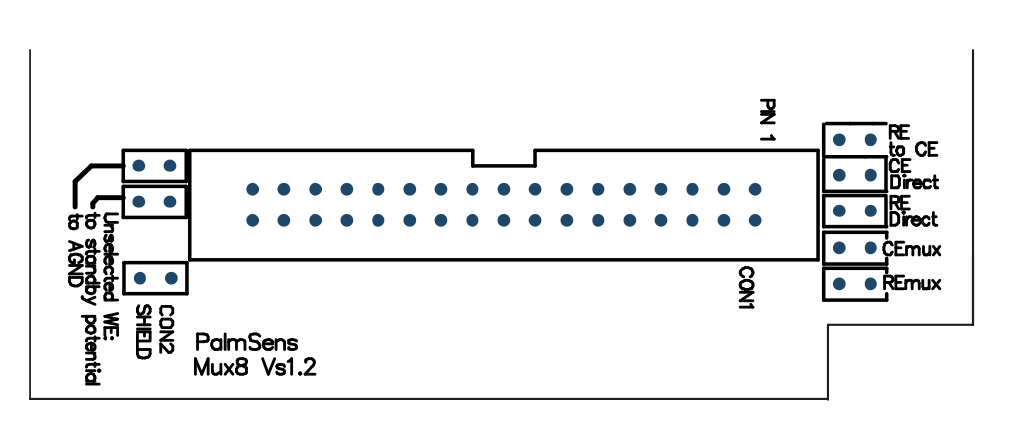
\includegraphics[width=0.45\columnwidth]{MUX_Pinout_Diagram}}	\\
\subfloat[EmStat with Multiplexer]{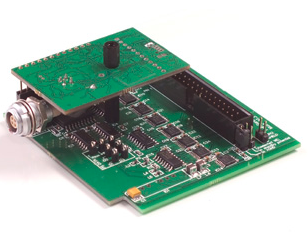
\includegraphics[width=0.45\columnwidth]{EmStat_with_Multiplexer}}	\quad
\subfloat[Pinout Schematic]{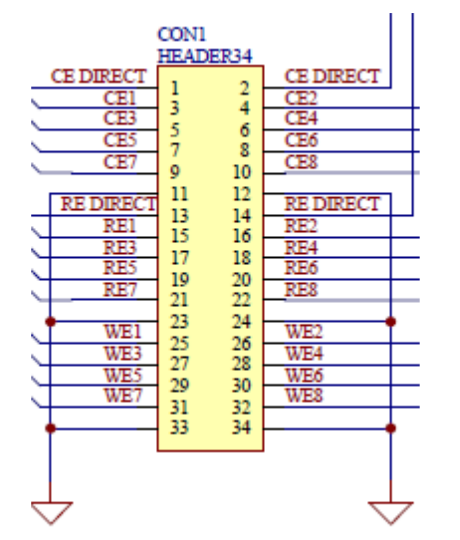
\includegraphics[width=0.45\columnwidth]{MUX_Pinout_Schematic}}
\caption{EmStat and Multiplexer from PalmSens \cite{mux-documentation}}
\label{emstat}
\end{figure}

The external interface from the Multiplexer is a standard 0.1" header but the sensors are made to be inserted into a USB receptacle.
To make this simple for the end user,
a custom breakout board was made to fit in the space between the EmStat and Multiplexer boards;
see figure \ref{breakout-board-sandwich}

\begin{figure}[tb]
\centering
\subfloat[Breakout Board]{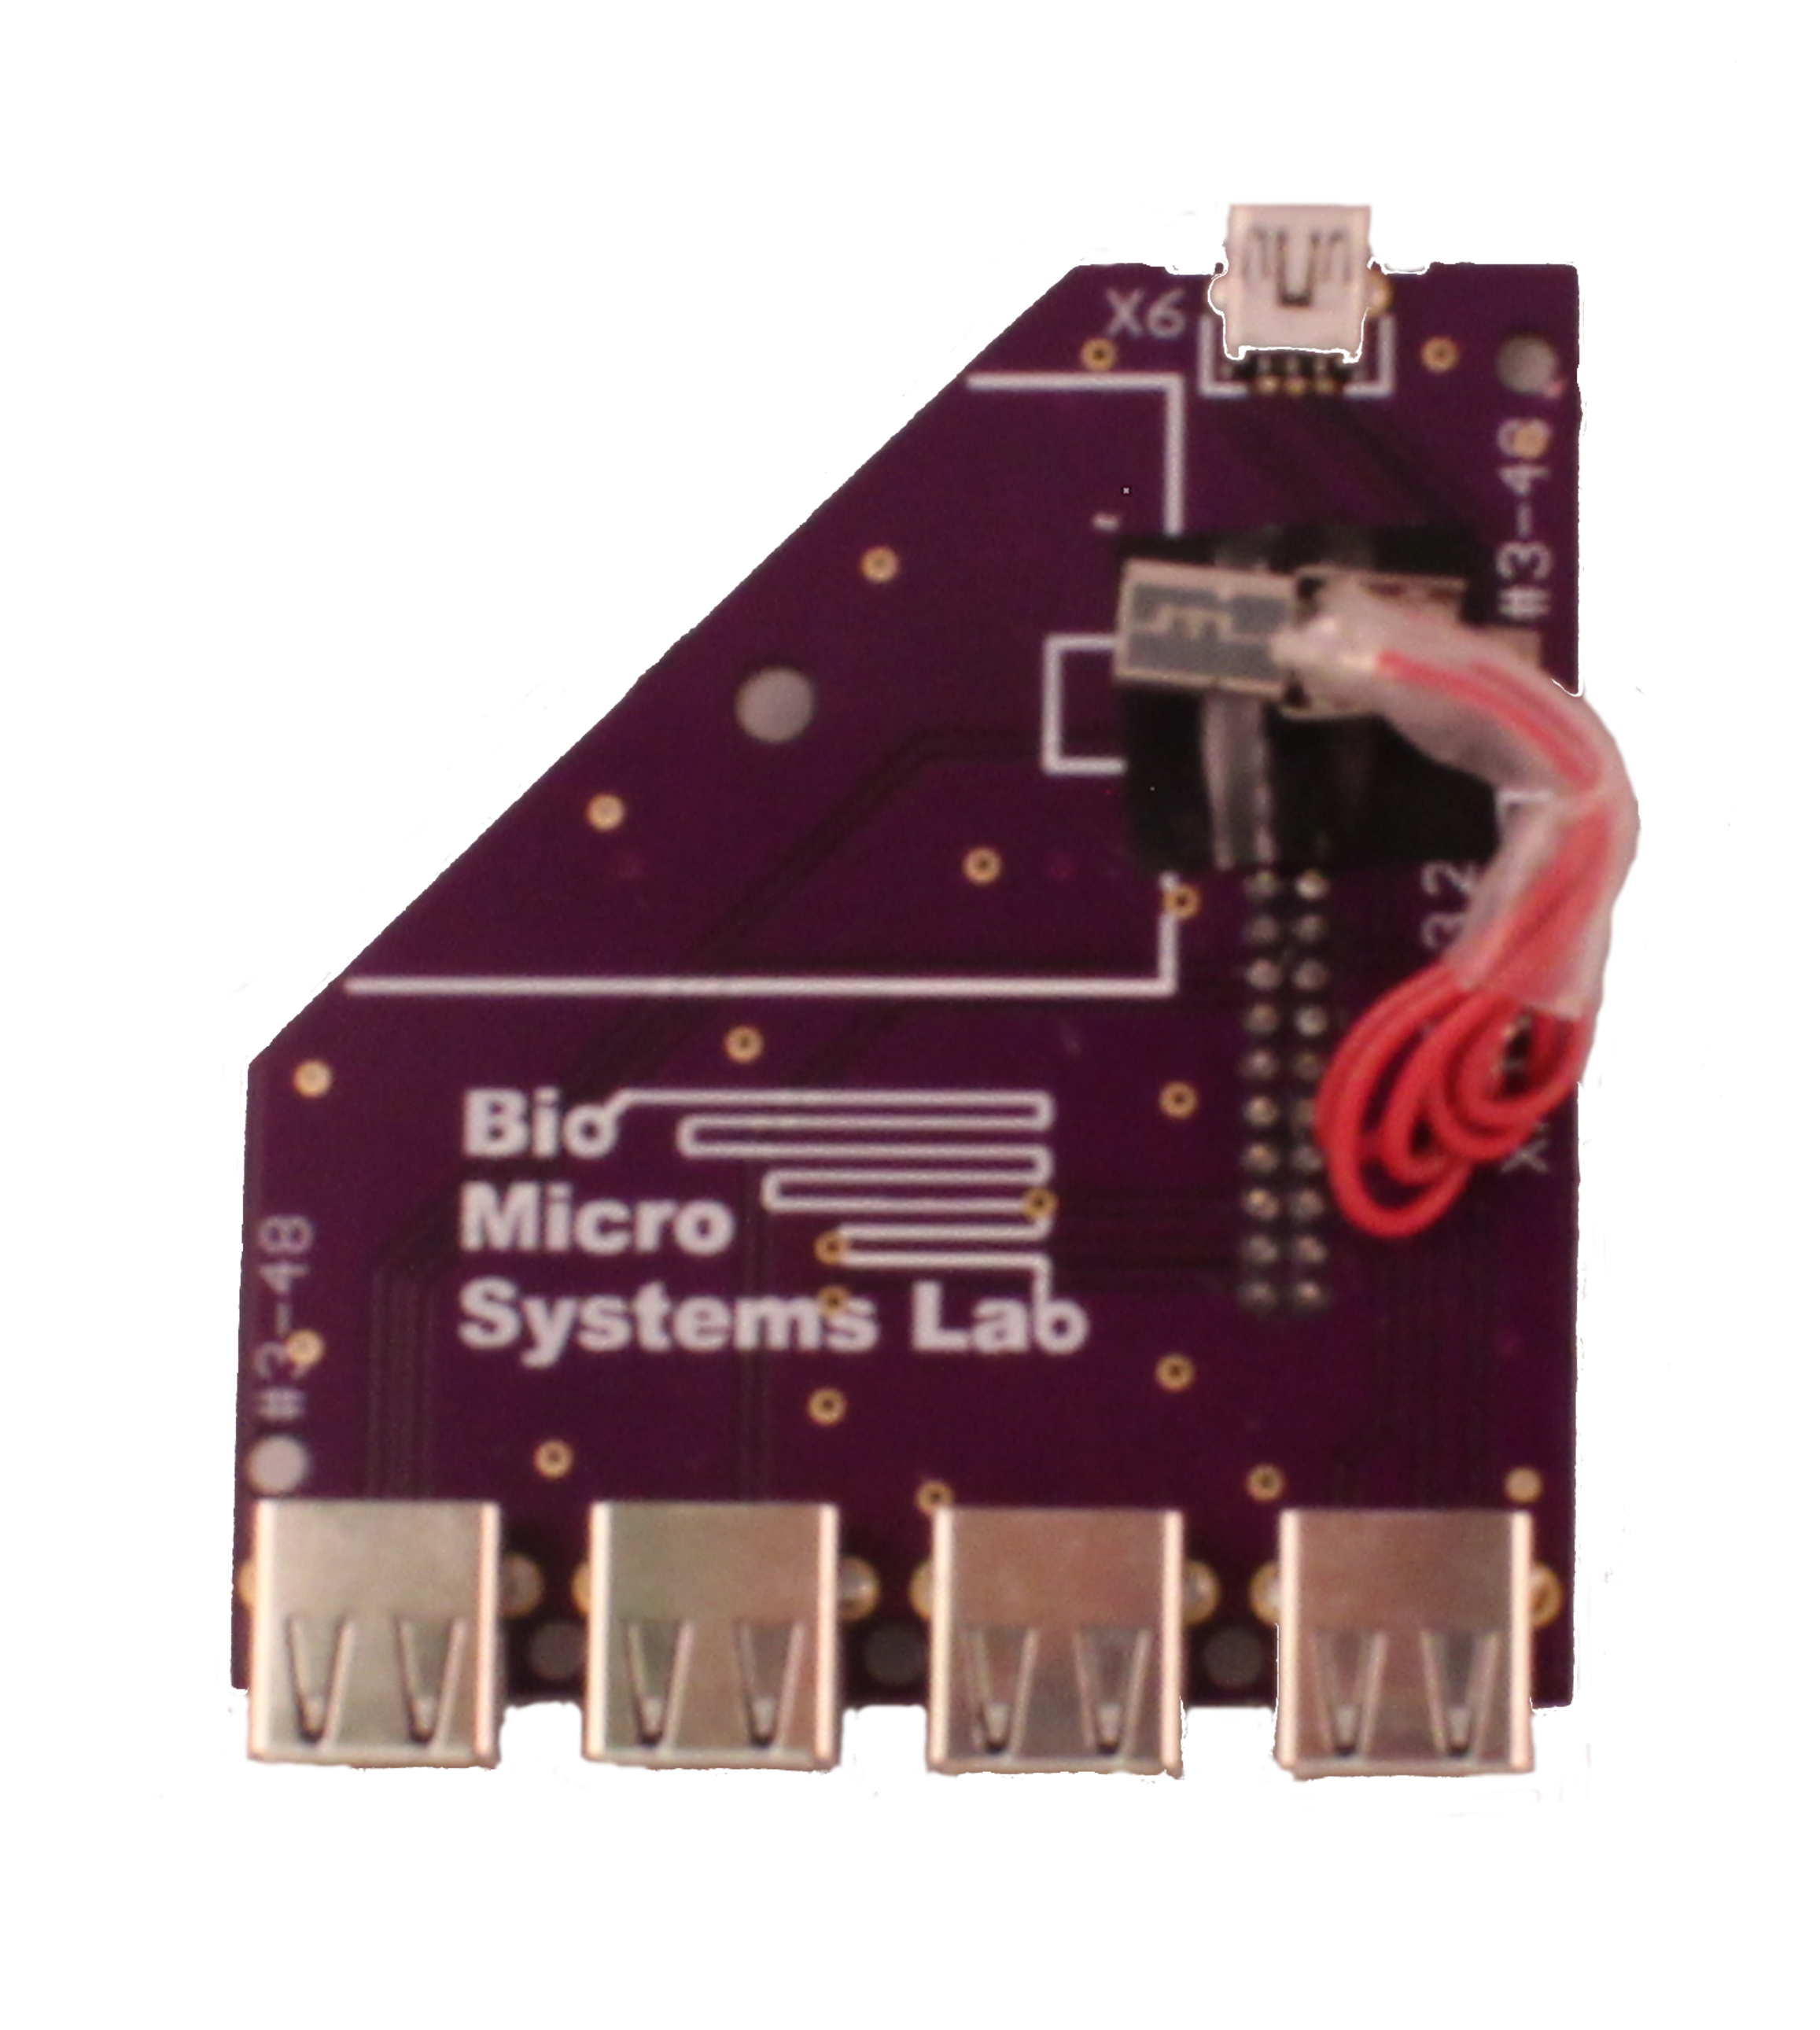
\includegraphics[width=0.4\columnwidth]{breakout-board}}	\quad
\subfloat[PCB Sandwich...tasty]{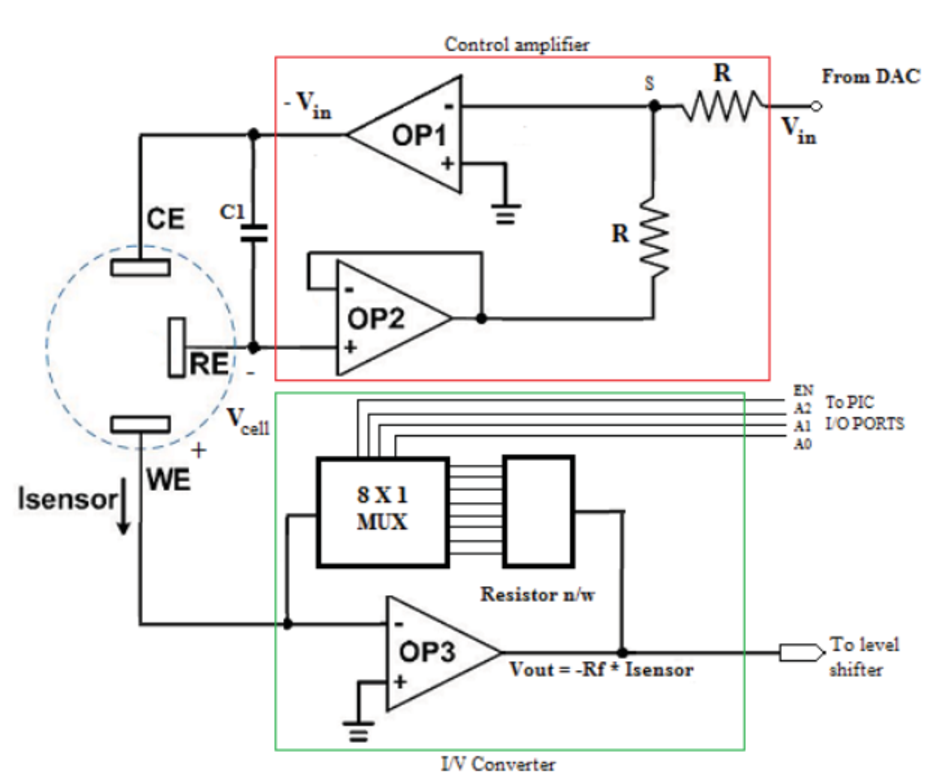
\includegraphics[width=0.5\columnwidth]{three-board-assembly}}
\caption{Breakout Board fits between EmStat and MUX}
\label{breakout-board-sandwich}
\end{figure}

The breakout board was designed in CadSoft Eagle and the \texttt{.brd} file was sent to OSH Park LLC for manufacture.
The Eagle project and part libraries used can be found in the directory \texttt{PCB\_Boards/}.
In addition to the manufactured board, the components listed in table \ref{breakout-board-bom} are need for assembly.

\begin{table}[ht]
\centering
\caption{Breakout Board Components}
\resizebox{\columnwidth}{!}{
\begin{tabular}{c | l | c}
\hline\hline
Qty.	&	Component	&	Man. Part \#	\\
\hline
4	&	USB type-A receptacle	&	292303-1	\\
1	&	USB mini receptacle	&	0548190519	\\
1	&	USB mini plug kit	&	1734205-1	\\
1	&	34-pin, 0.1" header	&	SFH11-PBPC-D17-ST-BK	\\
\hline
	&	hookup wire	and heat shrink&	\\
	&	for USB plug kit	&	\\
\hline\hline
\end{tabular}
} % end resize box
\label{breakout-board-bom}
\end{table}

The x-y coordinates used in aligning the EmStat, Multiplexer, and breakout board are shown in appendix \ref{x-y-coordinates-appendix}.
The schematic diagram for the breakout board and a transparent view from Eagle are incluced in appendices \ref{breakout-board-schematic} and \ref{breakout-board-top-view}

The packaging was designed in SolidWorks to be 3D-printed in two parts: a base and a lid.
In addition to the base and lid, six size \#3-48, 1.25" long machine screws and \#3-48 tapping equipment are needed for assembly.
Instructions for tapping can be found in appendix \ref{tapping-appendix}.

\begin{table}[ht]
\centering
\caption{Assembly Components}
\resizebox{\columnwidth}{!}{
\begin{tabular}{c | l | c}
\hline\hline
Qty.	&	Component	&	McMaster Part \#	\\
\hline
6	&	3-48, 1.25" socket head cap screws	&	90044A243	\\
\hline
	&	3-48 tap, tap driver, and spring	&	\\
	&	loaded tap guide	&	appendix \ref{tapping-appendix}	\\
\hline\hline
\end{tabular}
} % end resize box
\label{breakout-board-bom}
\end{table}

The design of the packaging was tested and iterated in house using a Makerobt Replicator 2X with ABS filament.
Mechanical drawings of the base and lid and a list of revisions are included in appendix \ref{enclosure-drawings-appendix}.

For printing with MakerBot or an outside printing house,
the files \texttt{Enclosure\_Base.STL} and \texttt{Enclosure\_Lid.STL} are needed from the \texttt{Packaging/} directory.
For editing the parts, the SolidWorks files are located in the \texttt{Packaging/SolidWorks\_Files} subdirectory.

In addition to the potentiostat system, three small sensor interface boards were built.
One allows a USB-style sensor to be extended away from the potentiostat system by a USB male-A-to-male-mini cable.
Another allows USB-style sensors to be easily connected to the WaveNow potentiostat.
The third allows USB-style sensors to be connected to aligator clips for electroplating, etc.

\begin{figure}[ht]
\centering
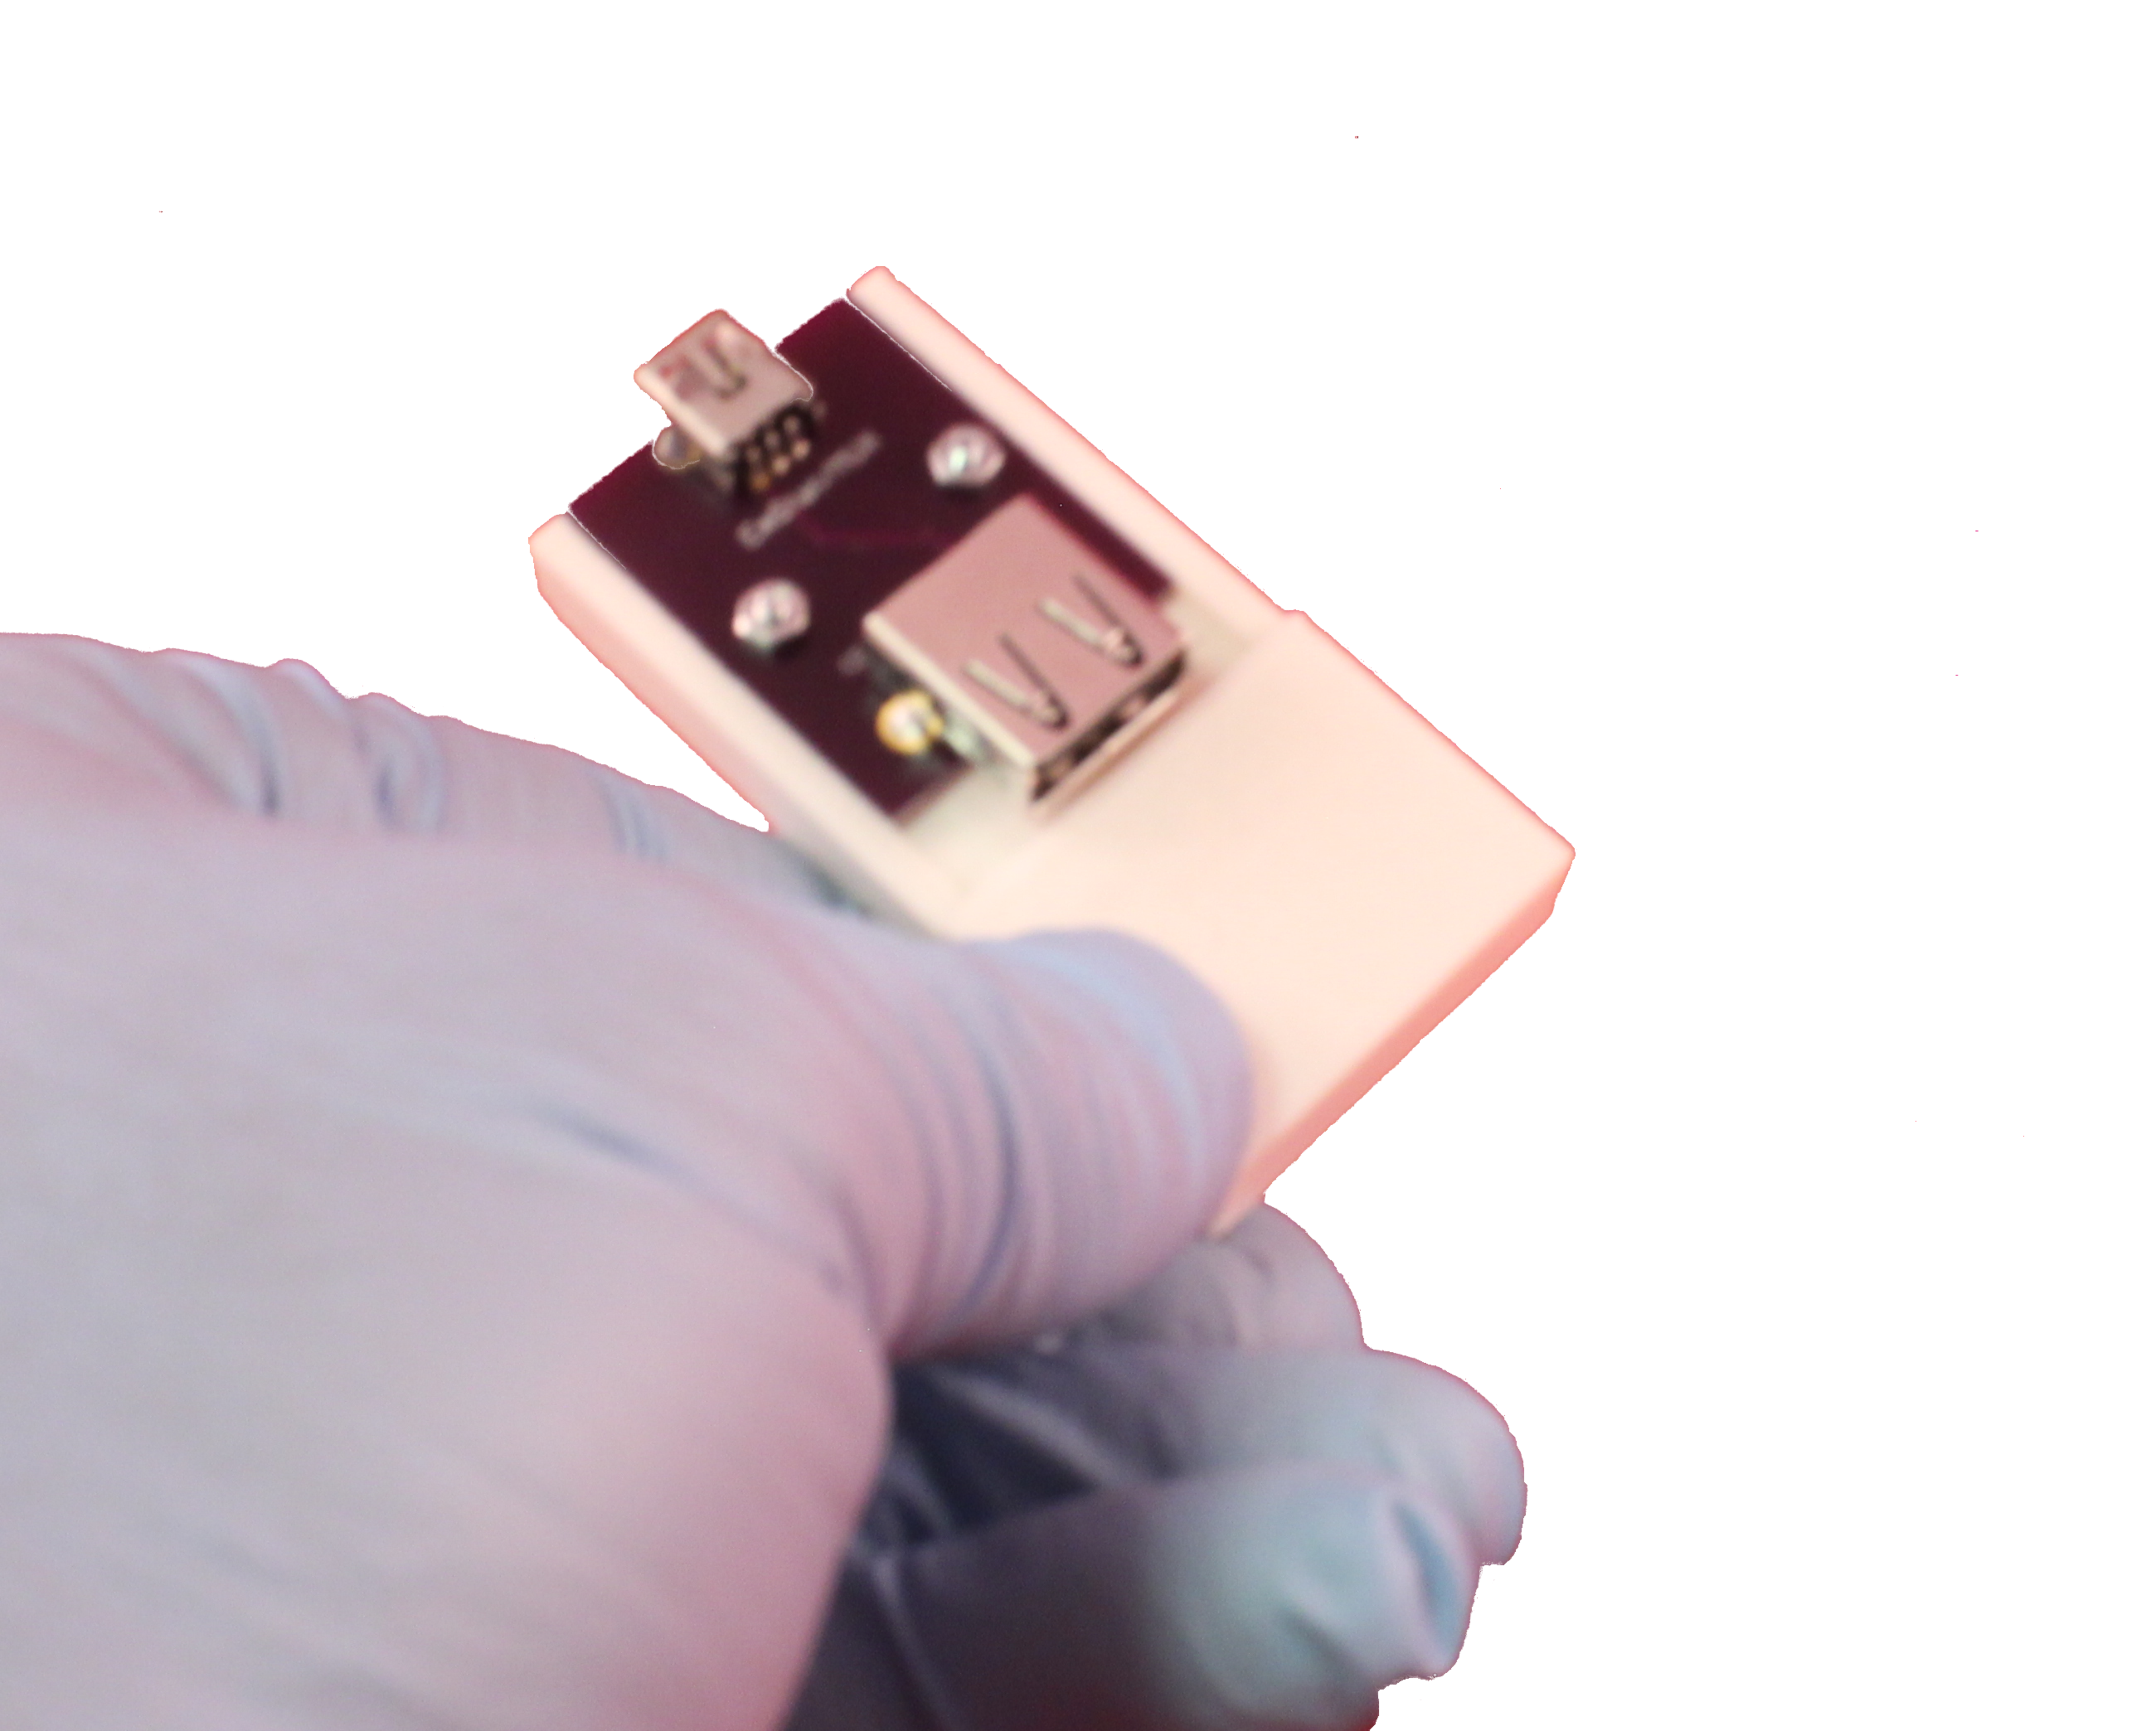
\includegraphics[width=0.4\columnwidth]{interface-board}
\caption{1 of 3 Sensor Interface Boards}
\end{figure}

\newpage
%------------------------------------------------

\section*{Results}

The enclosure base and lid were printed several times in house on the MakerBot and once outside by Shapeways.
Printing with Shapeways cost ~\$60 and had a lead time of three weeks.
However, the result was a much nicer product, as shown in figure \ref{print-comparison}.

\begin{figure}[ht]
\centering
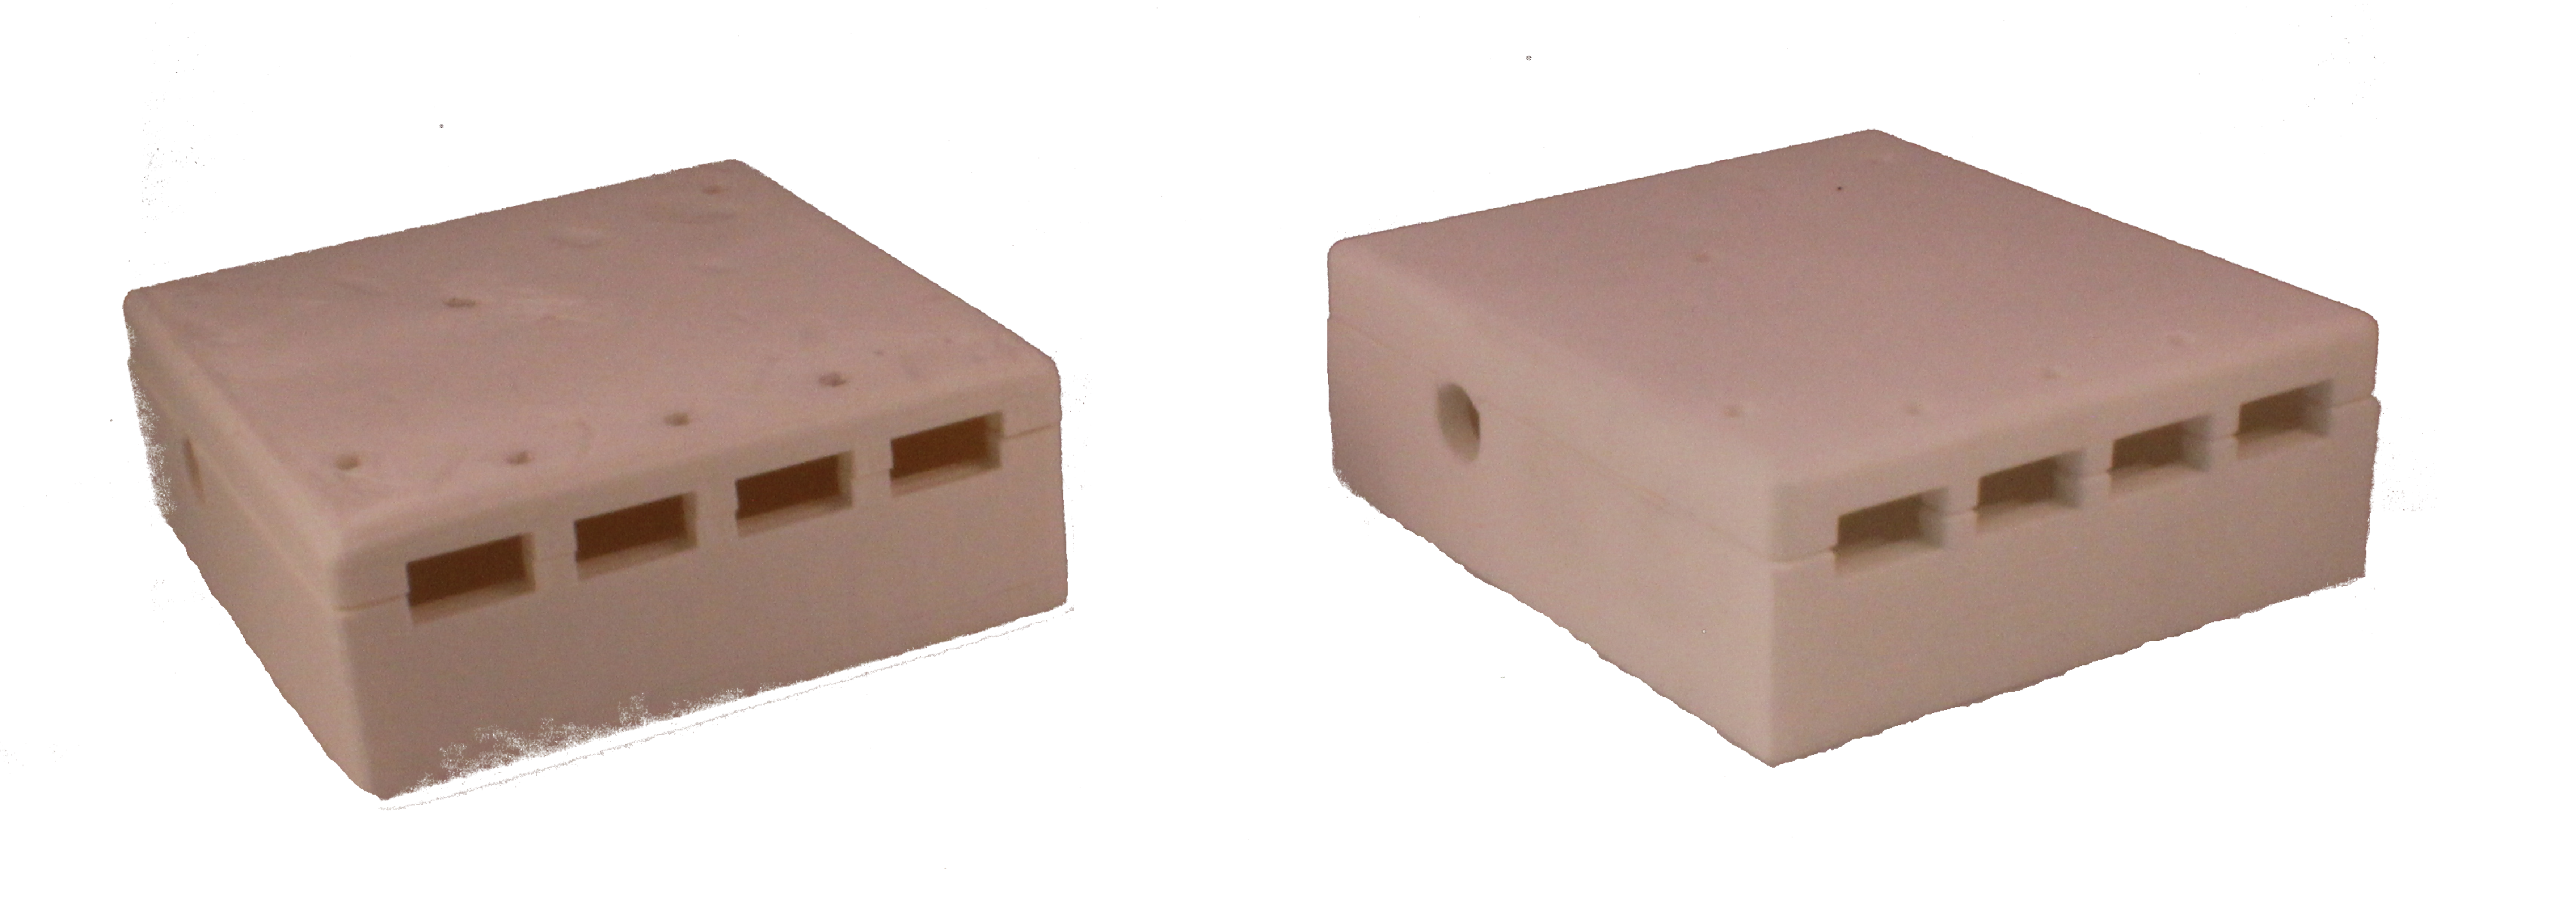
\includegraphics[width=1\columnwidth]{packaging-comparison}
\caption{Packaging Printed on MakerBot (left) and by Shapeways (right)}
\label{print-comparison}
\end{figure}

The parts printed by Shapeways had much more precision than the MakerBot,
to the extent that no hand filing or drilling had to be done just to get the parts to fit together.
The surface finish was also many times better.

Furthermore, tapping will be significantly better with the Shapeways base because the tolerance
for the through hole is much tighter and the enclosure is not hollow beyond the cylindrical face.

\section*{Conclusions}

All of the goals of the hardware are met by assembling the breakout board and 3D-printed
enclosure with the EmStat and Multiplexer boards from PalmSens.
For a higher quality product, it is recommended that the enclosure be reprinted
by an outside printing service such as Shapeways.

%------------------------------------------------

\newpage
\section*{Appendices}

The following are attached:
\begin{enumerate}
\item Tapping Instructions
\label{tapping-appendix}
\item X-Y Alignment of the EmStat, Multiplexer, and Breakout Boards
\label{x-y-coordinates-appendix}
\item Breakout Board Schematic Diagram
\label{breakout-board-schematic}
\item Breakout Board Top View
\label{breakout-board-top-view}
\item Enclosure Drawings--Including Revision History
\label{enclosure-drawing-appendix}
\item Interface Boards
\label{interface-boards-appendix}
\end{enumerate}

%------------------------------------------------

\section{Tapping Instructions}

The base part of the enclosure needs to be tapped six times--once for each assembly screw.
The screws have 3-48 threading,
which means they have an outermost diameter of 0.099" with 48 threads per inch.

The machine shop in 407 Rhodes has all of the tapping equipment needed.
Ron Hudepohl is very helpful and can show you where all the equipment is.

\begin{figure}[ht]
\centering
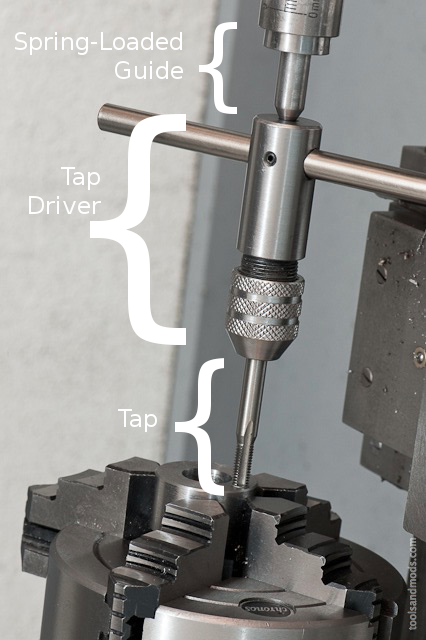
\includegraphics[width=0.7\columnwidth]{tapping-equipment}
\caption{Equipment for Tapping}
\end{figure}

It is much better to go to the shop than to purchase the tapping equipment because tapping
is easier if you can mount the enclosure and keep the tap vertically aligned.

If you mount the base part on mill with a digital x-y readout, figure \ref{tap-locations} will help.

\begin{figure}[ht]
\centering
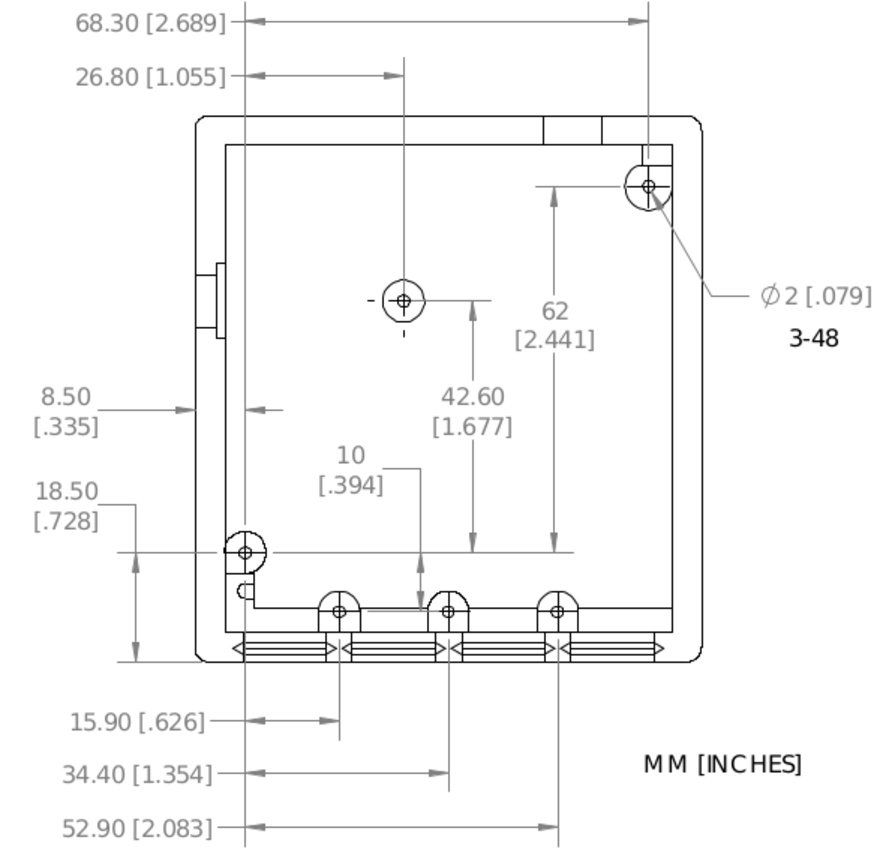
\includegraphics[width=0.9\columnwidth]{tap-location-drawing}
\caption{Coordinates for Tapping}
\label{tap-locations}
\end{figure}

%----------------------------------------------------------------------------------------
%	REFERENCE LIST
%----------------------------------------------------------------------------------------

\begin{thebibliography}{99} % Bibliography - this is intentionally simple in this template

\bibitem[Kang et al., 2014]{bms-article}
Wenjing Kang, Xing Pei, Adam Bange, Erin Haynes, William Heineman, and Ian Papautsky.
\newblock Copper-Based Electrochemical Sensor with Palladium Electrode for Cathodic Stripping Voltammetry of Manganese
\newblock {\em Analytical Chemistry}, 2014, 86, 12070--12077.

\bibitem[Sukhavasi, S., 2011]{zinc-masters-defense}
Sowmya Sukhavasi.
\newblock Zinc Chip Reader for Point-Of-Care Quantification of Zinc in Blood Serum
\newblock {\em University of Cincinnati}, Master's Thesis, 2011.

\bibitem[PalmSens, 2014]{mux-documentation}
PalmSens Compact Electrochemical Interfaces.
\newblock EmStat$^{3}$ Connecting to MUX8
\newblock {\em PalmSens Compact Electrochemical Interfaces}, Product Documentation, Revision: July 2014.

\end{thebibliography}

%----------------------------------------------------------------------------------------

\end{document}
